\section{\Glsfmtlong{wot}}\label{sec:wot}

Ein Problem bei der Service Discovery im \gls{iot} sind immer die Interoperabilität und Kompatibilität zwischen verschiedenen Systemen. Ein Bereich, in dem diese Aspekte von großer Relevanz sind, ist das Internet. Webtechnologien müssen für eine Vielzahl von Geräten und Anwendungen funktionieren. So wurde das Internet auch als Inspirationsquelle für die Lösung solcher und anderer Probleme im \gls{iot} genutzt. Diese Kombination wird im Allgemeinen als \gls{wot} bezeichnet.

Das \gls{wot} ist eine Erweiterung des \gls{iot}, die grundsätzlich die \glspl{thing} (oder deren \glspl{intermediary}) um eine Web-Server-Komponente erweitert, mit der Kommunikation von außen über einen \gls{uri} oder \gls{iri} initialisiert und durchgeführt werden kann.

Im Laufe der Jahre haben sich dabei die \glsxtrshort{wot}-Spezifikationen und -Empfehlungen des \gls{w3c}[s], welches auch die Spezifikationen für andere Webtechnologien herausbringt, zu den meistgenutzten und vollständigsten entwickelt \autocite[vgl.][47573]{Sciullo.2022.ASotWoT}, weshalb diese in den nachfolgenden Unterkapiteln näher betrachtet werden.

Es gibt verschiedene Spezifikations- und Richtliniendokumente, die das \gls{w3c} bereitstellt.

\begin{itemize}
  \item Die \emph{Architecture} \autocite{w3c.wot.architecture.20200408} gibt einen Überblick über das \gls{wot}, welches vom \gls{w3c} standardisiert bzw.\ empfohlen wird.
  \item Die \emph{\glsfmtlong{td}} \autocite{w3c.wot.td.20200623} ist die Spezifikation für das Format, in dem einzelne \glspl{wt} beschrieben werden.
  \item Die \emph{Binding Templates} \autocite{w3c.wot.bt.20200130} sind Richtlinien, wie Netzwerkschnittstellen definiert werden sollen.
  \item Die \emph{Scripting API} \autocite{w3c.wot.scriptingapi.20201124} beschreibt eine (optionale) JavaScript-API, die für eine Anwendung genutzt werden kann, die auf das \gls{wot} zugreifen können soll.
  \item Die \emph{Discovery} \autocite{w3c.wot.discovery.20210602} beschreibt, wie sich sowohl \glspl{thing} nach außen bekannt machen können, als auch Anwendungen nach existierenden \glspl{thing} erkundigen können. Zum Zeitpunkt der Erstellung dieses Berichts ist dieses Dokument jedoch noch nicht in einem fertigen Zustand gewesen.
  \item Die \emph{Security und Privacy Guidelines} \autocite{w3c.wot.spg.20191106} enthalten Richtlinien zur sicheren Implementierung und Konfiguration von \glspl{thing} sowie möglicherweise auftretende Probleme und deren Behebung.
\end{itemize}

Es gibt noch weitere Dokumente, die jedoch nicht relevant für den Anwendungszweck der Service Discovery sind und daher hier nicht angeführt werden. Sie können unter \url{https://www.w3.org/TR/?tag=wot} eingesehen werden.

\subsection{Architekturüberblick}\label{subsec:wotarchitecture}

Für das \gls{wot} gibt es verschiedenste Anwendungsfälle. All diese haben Gemeinsamkeiten und Unterschiede, aus denen sich die Anforderungen an eine \glsxtrshort{wot}-Architektur \autocite[vgl.][]{w3c.wot.architecture.20200408} ergeben.

\begin{figure}[H]
  \centering
  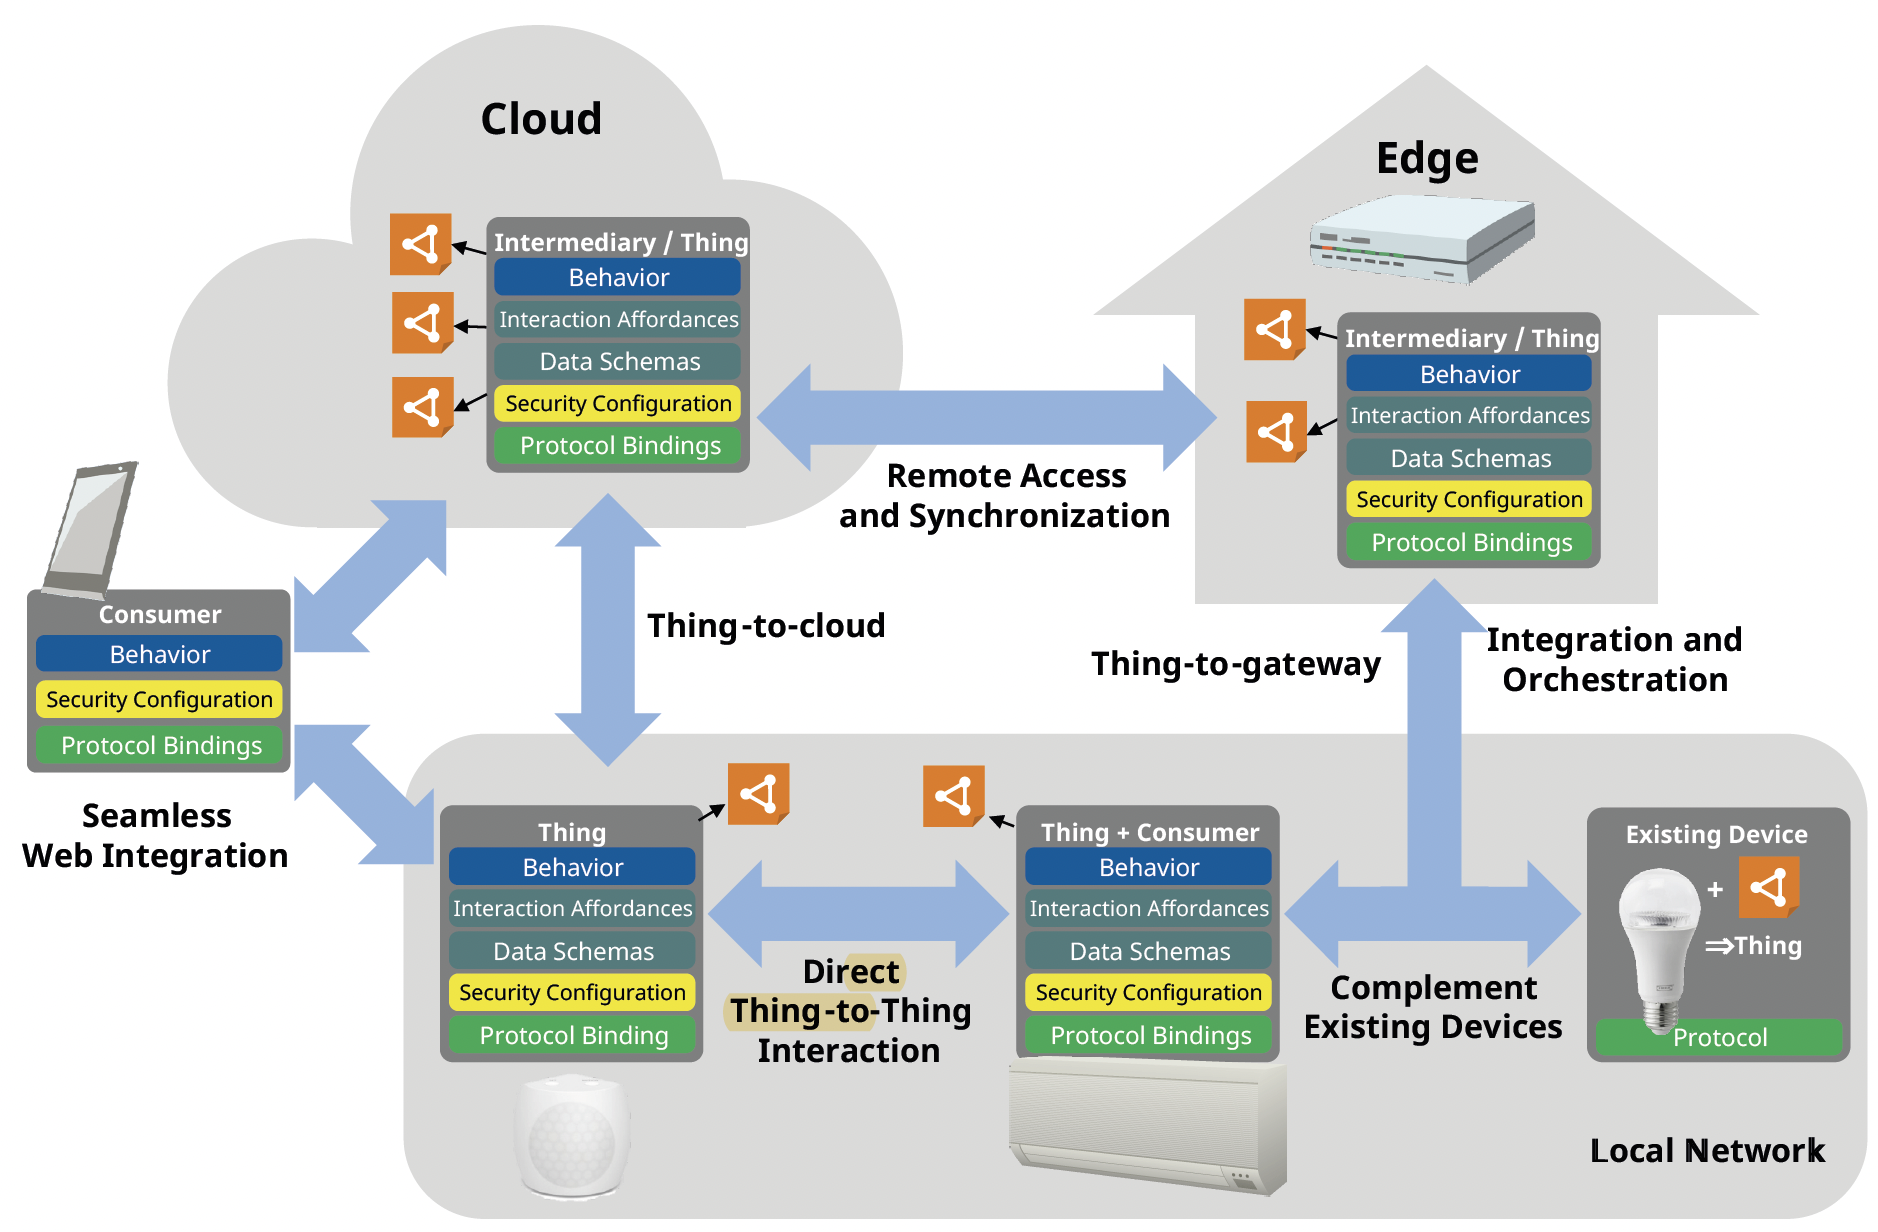
\includegraphics[width=12cm]{abstract-architecture-overview.png}
  \caption{\glsxtrshort{wot}-Architektur}\label{fig:wot_abstract_architecture}
\end{figure}

% Problem Heterogenität

Durch die starke Heterogenität der Anwendungen und Geräte, aber auch der bereits existierenden \glsxtrshort{iot}-Systeme, entsteht eine Vielzahl von Anforderungen. Diese lassen sich häufig in zwei Kategorien einteilen: Positive Anforderungen, die in allen betroffenen Entitäten umgesetzt werden können, oder negative Anforderungen, die nicht in allen betroffenen Entitäten umgesetzt werden können und wodurch die Anforderung aus einer Unabhängigkeit von diesem Teilaspekt besteht. Im Zentrum stehen vier Kernelemente: Flexibilität, Kompatibilität, Skalierbarkeit und Interoperabilität.

% Hardware

Die Architektur muss demnach hardwareunabhängig sein. Auch bestimmte Technologien können nicht vorausgesetzt werden, denn es muss Kompatibilität zu allen vorhandenen Geräten und Systemumgebungen sichergestellt werden. Dadurch fokussiert sich das \gls{wot} des \gls{w3c}[s] auf höhere Systemebenen und somit vor allem die Kommunikationsebene.

% Web Thing

Auf dieser Basis wird die Architektur eines \gls{wt}[s] in verschiedene Bereiche unterteilt. Neben dem eigentlichen \emph{Verhalten} sind das \emph{Interaktionsaffordanzen}, die dazugehörigen \emph{Datenschemata}, die \emph{Sicherheitskonfiguration} und \emph{Protokollbindungen}. Dabei sind die Protokollbindungen die Definition, wie konkret Interaktionen durchgeführt werden können, während die Affordanzen nur beschreiben, was möglich ist, unabhängig von Protokollen oder Datenkodierung. Das \emph{Interaktionsmodell} beschreibt dabei neben Navigation drei weitere Typen von Interaktionsaffordanzen:

\begin{itemize}
  \item \emph{Eigenschaften} bilden den Zustand eines \gls{thing}[s] ab.
  \item Mittels \emph{Aktionen} kann der Zustand eines \gls{thing}[s] oder eine Funktion auf diesem geändert bzw.\ aufgerufen werden. % TODO: Aktionen
  \item \emph{Ereignisse} finden bei Zustandsänderungen statt und können Daten asynchron an \gls{consumer} senden.
\end{itemize}

Dabei werden die einzelnen Interaktionsschnittstellen durch Verknüpfungen in Form von \gls{uri}[s] und optionale Zusatzbeschreibungen maschinenlesbar definiert.

\begin{figure}[H]
  \centering
  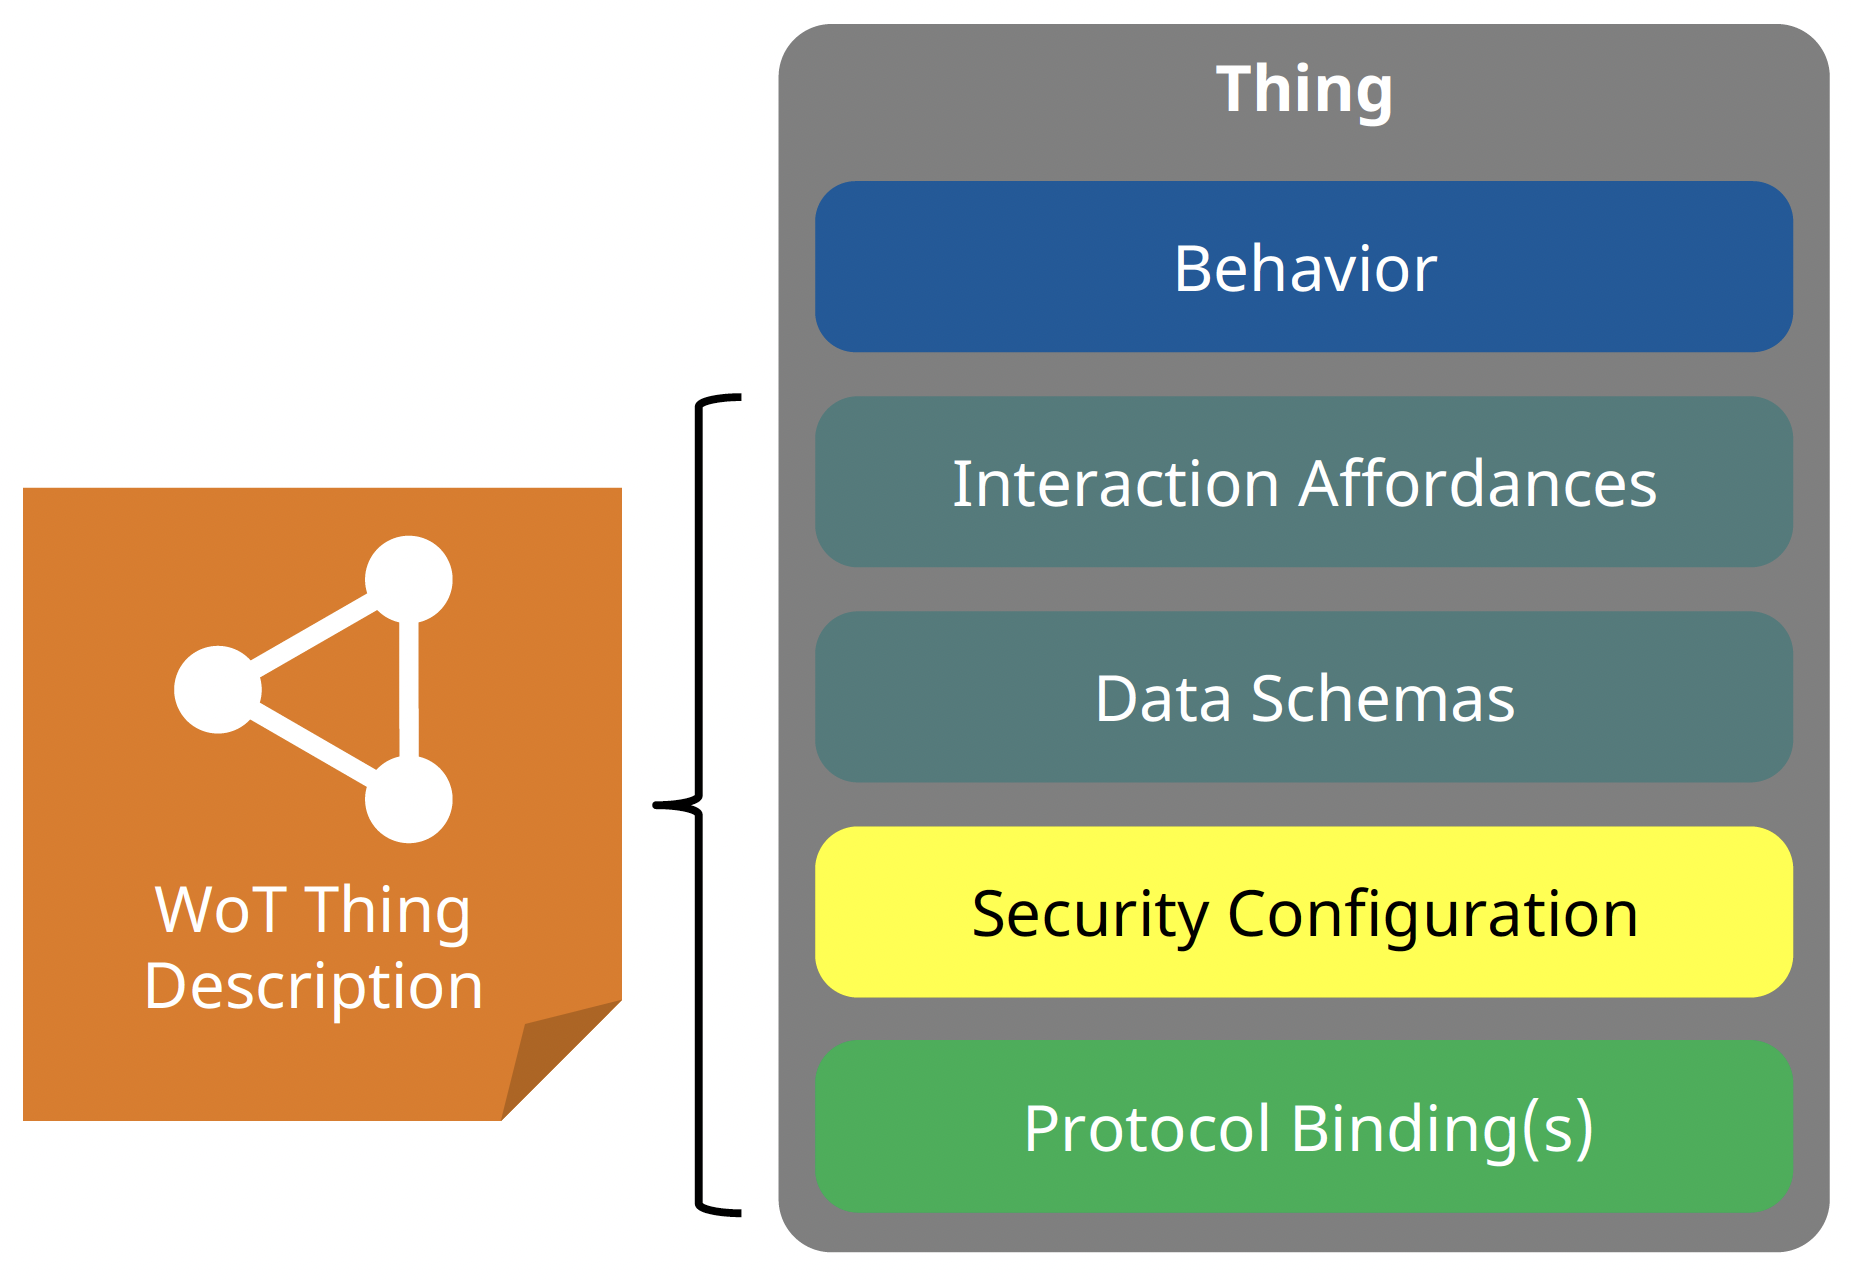
\includegraphics[width=8cm]{thing-architecture.png}
  \caption{\gls{thing}-Architektur}\label{fig:td_thing_architecture}
\end{figure}

% Thing-Beschreibung

Jedes \gls{thing} (oder dessen \gls{intermediary}) muss diese Funktionalitäten und Metadaten über sich bereitstellen können. Dazu gehören die bereits erwähnten Interaktionsaffordanzen, Datenschemata, die Sicherheitskonfiguration und die Protokollbindungen, neben dem Namen oder der Version des \gls{thing}[s] aber nicht zuletzt auch verwandte \glspl{thing}. Diese Eigenschaften sollen sowohl menschenlesbar als auch maschinenlesbar sein, semantisch annotiert werden sowie, falls zutreffend, Internationalisierung unterstützen können. Die Beschreibung dieser Eigenschaften wird \gls{td} genannt. Die \gls{td} wird als \gls{json} übermittelt und dient als Einstiegspunkt für ein \gls{thing}.

Im Idealfall wird eine \gls{td} direkt auf dem jeweiligen \gls{thing} erstellt und bereitgestellt. Domänenspezifisches Vokabular wird dabei zwar nicht durch die \glsxtrshort{wot}-Spezifikationen des \gls{w3c} abgedeckt, da die \gls{td} aber \gls{jsonld} implementiert, kann beliebiges Vokabular als Kontext eingebunden werden. Eine genauere Beschreibung der \glsfmtlong{td} ist in \autoref{subsec:wottd} zu finden.

% Protokolle

\Glspl{wt} müssen verschiedene Protokolle unterstützen können. Dazu zählen nicht nur Internetprotokolle, sondern auch Protokolle, die im \gls{lan} genutzt werden. Außerdem sollten auch Kombinationen von Protokollen genutzt werden können. So soll grundsätzlich mit \glsxtrshort{rest}-\glsxtrshortpl{api} gearbeitet werden, jedoch soll auch der Datenaustausch mit dem \gls{pubsub}-Muster möglich sein.

% Discovery

Damit mit einem \gls{wt} -- also der Repräsentation eines \gls{thing}[s] im Web -- interagiert werden kann, muss ein \gls{consumer} aber von diesem wissen. Dafür muss nach dem \gls{wt} gesucht werden können. Diese Suche muss syntaktisch (Attribute, …) und semantisch (Funktionalitäten auf Basis eines einheitlichen Vokabulars) über verschiedene Formate möglich sein. Es kann hilfreich sein, für die Erkundung ein Verzeichnis zu nutzen, bei dem sich die einzelnen \glspl{wt} automatisiert oder manuell registrieren können und welches darauf basierende Suchanfragen bearbeiten kann. (Siehe dazu auch \autoref{subsec:wotdiscovery}.)

% Sicherheit

Die \gls{td} umfasst auch Angaben zur Sicherheit nach außen. Dazu gehören z.\,B.\ Authentifizierungsmethoden wie Basic oder OAuth2.0. Grundsätzlich sollten (laut der Spezifikation) \gls{td}[s] nur autorisierten Personen zugänglich gemacht werden, da die enthaltenen Metadaten potenziell sensible Informationen beinhalten können. Trotzdem -- oder gerade deswegen -- sollten die Personen, die \gls{td}[s] erstellen oder verwalten, darauf achten, dass nur öffentliche Sicherheitsinformationen -- wie die jeweilige Authentifizierungsmethode -- in einer \gls{td} vorkommen.

% Barrierefreiheit

Barrierefreiheit ist im Rahmen der Spezifikationen kein Thema, da es um die Kommunikation zwischen Anwendungen und Geräten geht und Personen nicht direkt auf das \gls{wot} zugreifen. Allerdings gilt es zu bedenken, dass mit entsprechenden Annotationen möglicherweise Code oder ganze Interfaces generiert werden könnten, sodass die Integration von Barrierefreiheit durchaus auch Auswirkungen auf andere Bereiche hätte.

Weitere Anforderungen, die jedoch nicht zur Thematik der Service Discovery beitragen, können in \citetitle{w3c.wot.architecture.20200408} \autocite{w3c.wot.architecture.20200408} nachgelesen werden.

\subsection{\Glsfmtlong{td}}\label{subsec:wottd}

Die \glsfirst{td} \autocite{w3c.wot.td.20200623} hat, wie in \autoref{subsec:wotarchitecture} bereits oberflächlich beschrieben, vier Hauptbestandteile:

\begin{itemize}
  \item Beschreibende Metadaten über das \gls{thing};
  \item Interaktionsaffordanzen, die beschreiben, wie man das \gls{thing} nutzen kann;
  \item Schemata, die beschreiben, wie die Daten aussehen (müssen), die entweder an das oder von dem \gls{thing} geschickt werden;
  \item Verweise auf verwandte \glspl{thing} oder Dokumente.
\end{itemize}

Eine \gls{td} wird in \glsxtrshort{json} verfasst und folgt dem \glsxtrshort{jsonld}-Standard. Dabei existieren verschiedene Vokabulare für die unterschiedlichen Bereiche des Informationsmodells, die als Kontext verwendet werden können.

Jedes Vokabular enthält im Grunde Definitionen von Datenstrukturen, die im objektorientierten Kontext als Objekte verstanden werden können. Das Kernvokabular definiert dabei den grundsätzlichen Aufbau einer \gls{td}, während es dabei die anderen spezifischeren Vokabulare für ihre jeweiligen Teilbereiche referenziert.

\subsubsection{Kernvokabular}

Das Kernvokabular deckt das Interaktionsmodell aus Eigenschafts-, Aktions- und Ereignisinteraktionsaffordanzen ab.

\begin{figure}[H]
  \centering
  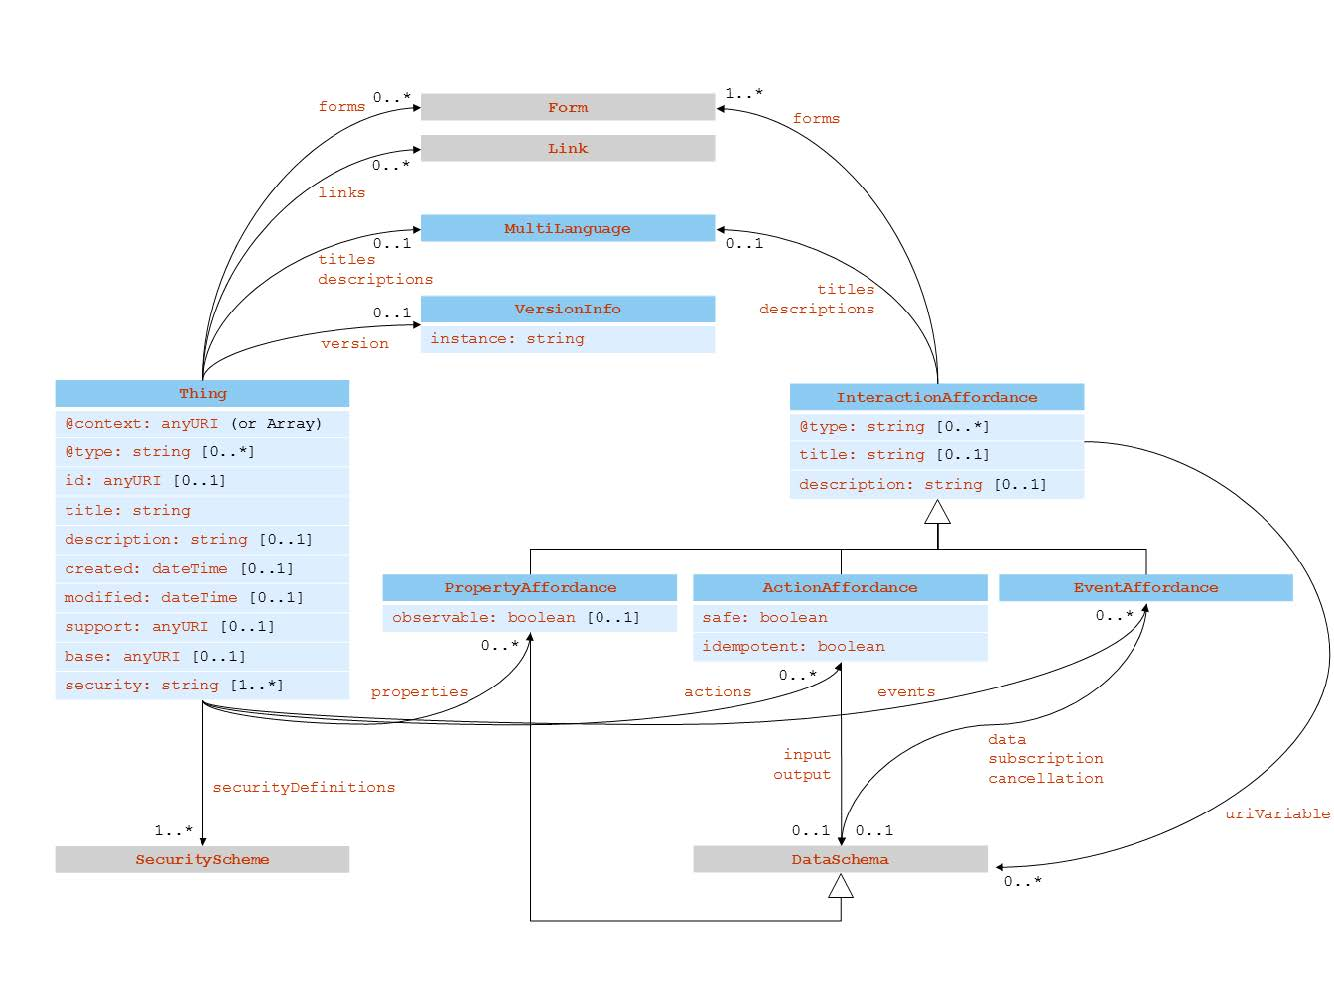
\includegraphics[width=\textwidth]{td-core-vocabulary.jpg}
  \caption{\glsxtrshort{td} Kernvokabular}\label{fig:td_core_vocabulary}
\end{figure}

Das \lstinline{Thing} ist dabei das Grundobjekt, welches die Wurzel eines \glsxtrshort{td}-Dokuments definiert. Dazu gehören der \gls{uri} des \gls{thing}[s], \glsxtrshort{jsonld}-Annotationen, Beschriftungen, Metadaten, vor allem aber die einzelnen Bereiche des Interaktionsmodells, Links zu anderen \glspl{thing}, Hypermediakontrolldefinitionen sowie Sicherheitsmechanismen des \gls{thing}[s].

Es gibt drei Arten von \lstinline{InteractionAffordance}s:

\begin{itemize}
  \item \lstinline{PropertyAffordance}s
  \item \lstinline{ActionAffordance}s
  \item \lstinline{EventAffordance}s
\end{itemize}

Allen ist gemein, dass sie Beschriftungen haben, Hypermediakontrollen, die beschreiben, wie mit ihnen interagiert werden kann, sowie Schemata für Werte, die übergeben werden müssen. Für eine \lstinline{PropertyAffordance} kann zusätzlich definiert werden, ob diese überwacht werden kann. Bei einer \lstinline{ActionAffordance} kann noch definiert werden, wie Eingabe- und Ausgabedaten aussehen sollen und wie sich die Aktion verhält. Bei einer \lstinline{EventAffordance} können stattdessen die Daten definiert werden, die bei der Abonnierung und Deabonnierung benötigt werden sowie die, die dann erhalten werden.

\subsubsection{Datenschemavokabular}

Das Datenschemavokabular leitet sich aus der JSON-Schema-Spezifikation \autocite{jsonschema} ab.

\begin{figure}[H]
  \centering
  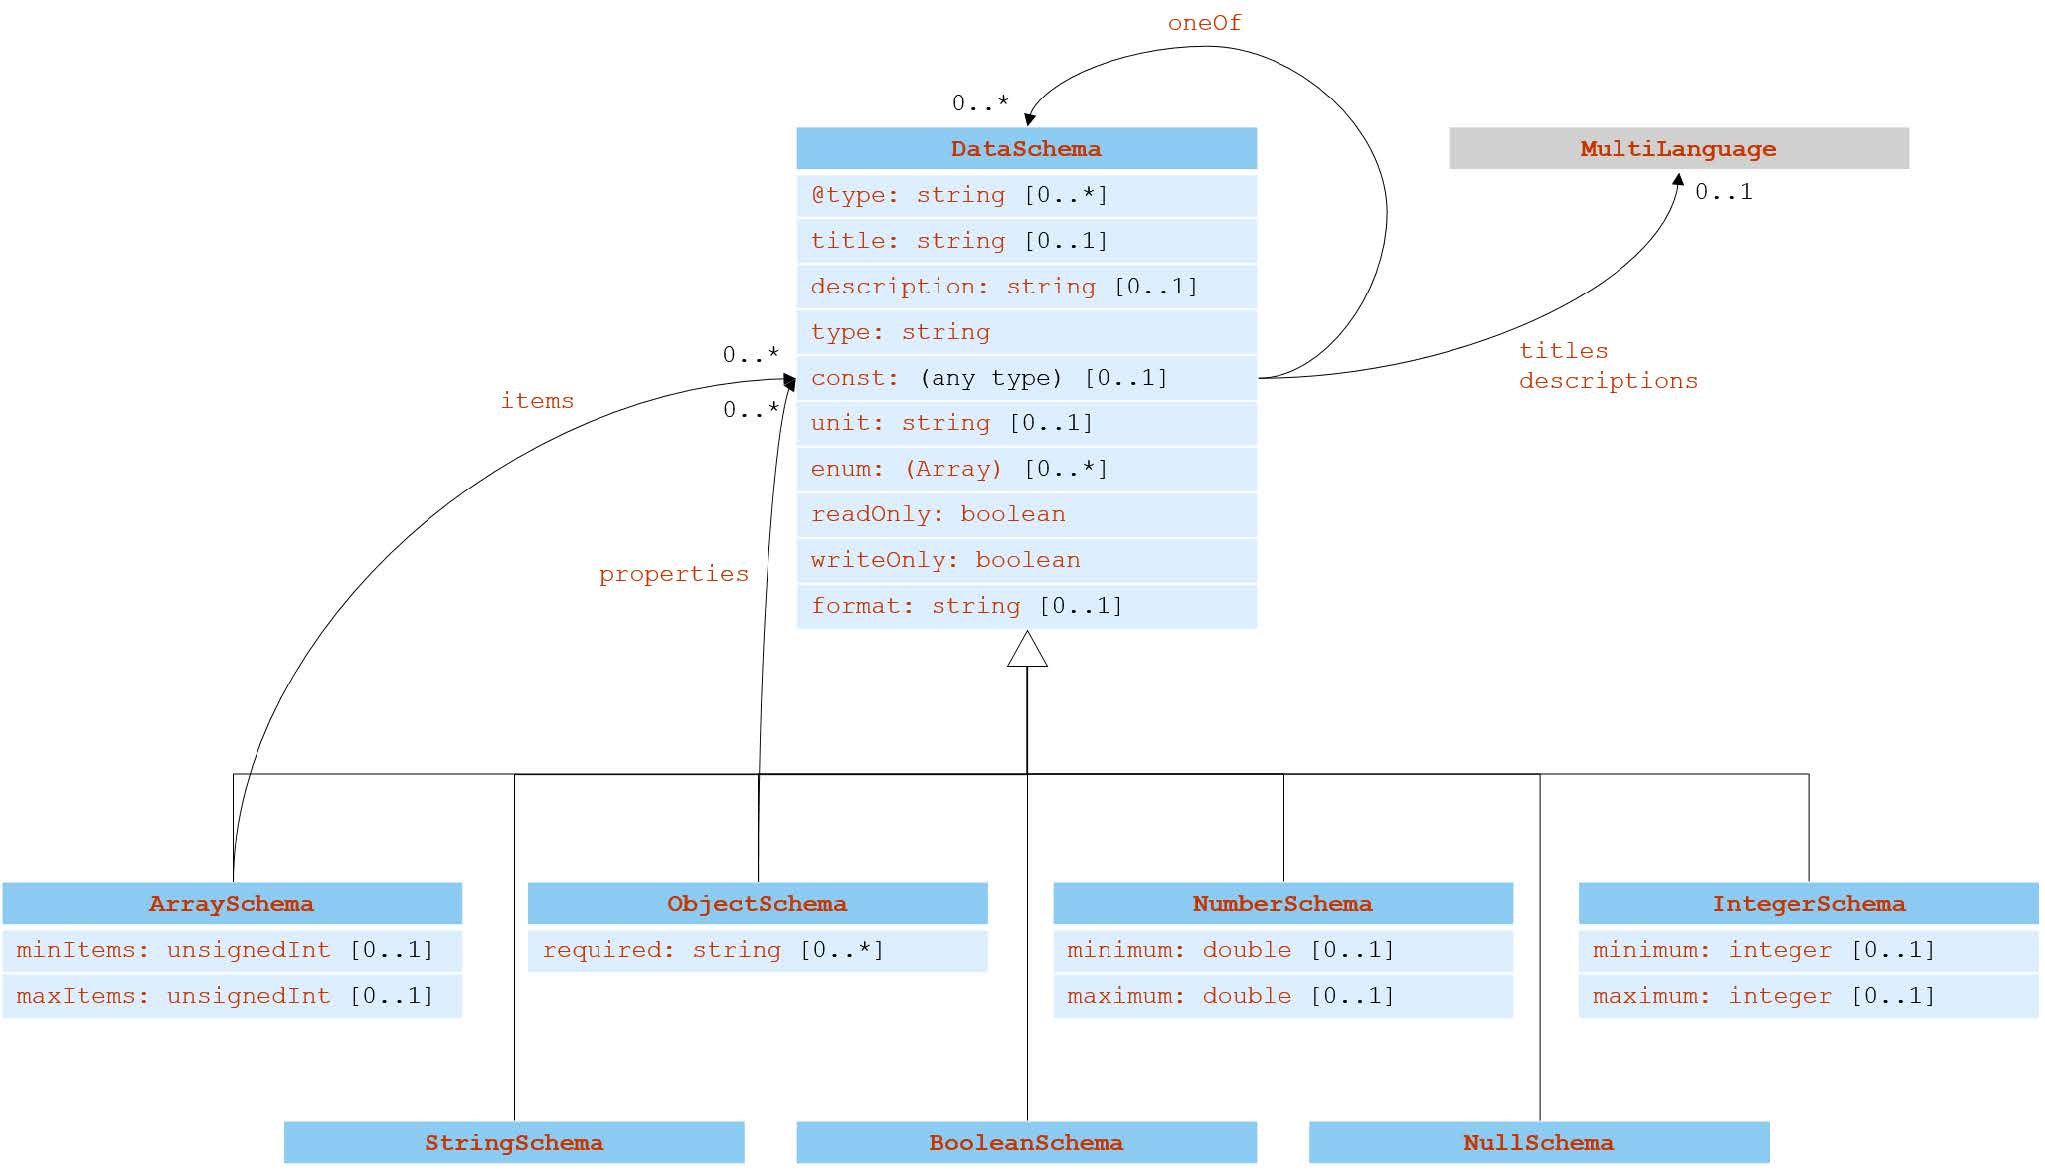
\includegraphics[width=\textwidth]{td-data-schema-vocabulary.jpg}
  \caption{\glsxtrshort{td} Datenschemavokabular}\label{fig:td_data_schema_vocabulary}
\end{figure}

\subsubsection{Sicherheitsvokabular}

Das Sicherheitsvokabular definiert Sicherheitsmechanismen und dessen Konfigurationen.

\begin{figure}[H]
  \centering
  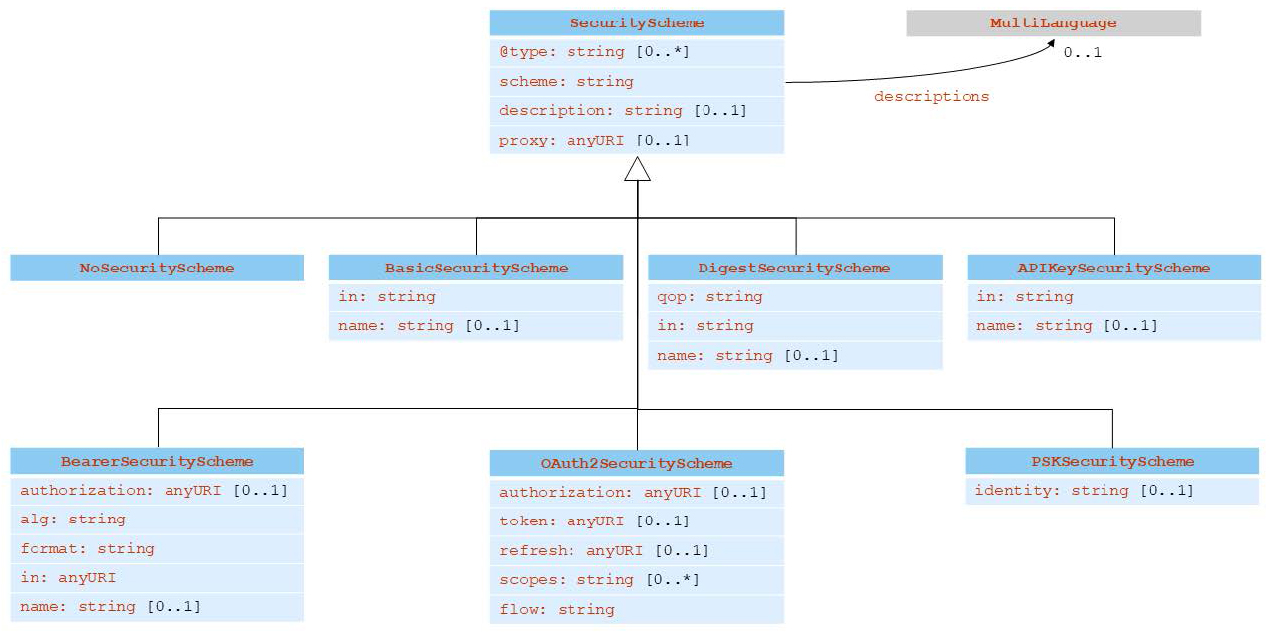
\includegraphics[width=\textwidth]{td-security-vocabulary.jpg}
  \caption{\glsxtrshort{td} Sicherheitsvokabular}\label{fig:td_security_vocabulary}
\end{figure}

Ein \lstinline{SecurityScheme} beinhaltet dabei grundsätzlich einen Bezeichner für das jeweilige Sicherheitsschema und möglicherweise Beschriftungen oder einen \glsxtrshort{uri}, auf die das Sicherheitsschema einen möglichen Zugriff definiert -- wenn es nicht um den aktuellen \glsxtrshort{uri} geht. Der Schemabezeichner wird dabei als Diskriminator für die einzelnen Sicherheitsschemata verwendet. Dabei sind je nach Sicherheitsschema weitere Objektattribute erforderlich oder möglich.

\subsubsection{Hypermediakontrollvokabular}

Das Hypermediakontrollvokabular definiert die Hauptbestandteile von Kommunikation über \gls{rest} mit Verweisen und Formularen.

\begin{figure}[H]
  \centering
  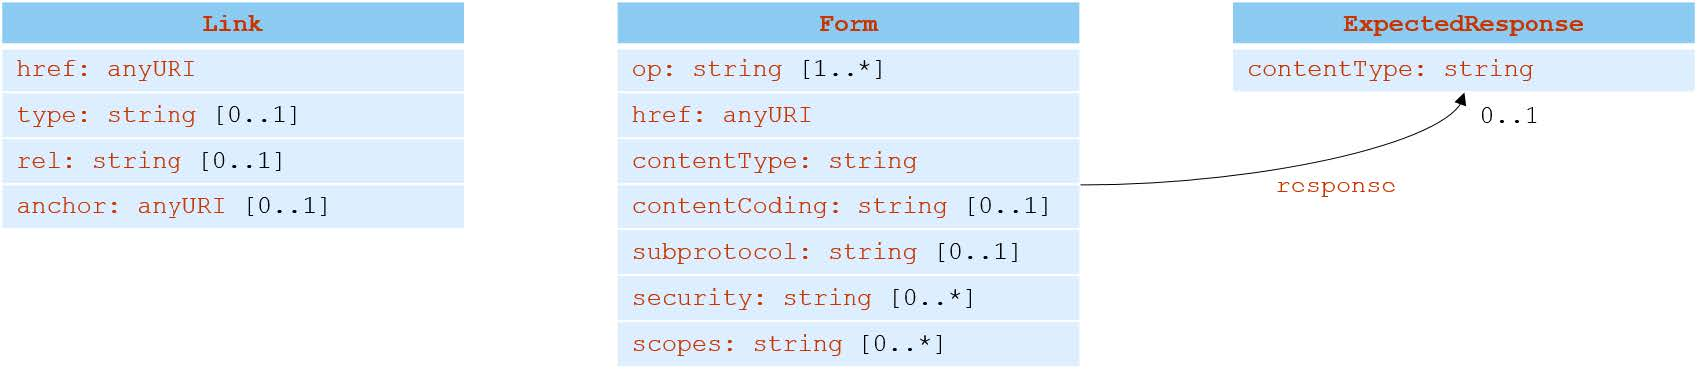
\includegraphics[width=\textwidth]{td-hypermedia-controls-vocabulary.jpg}
  \caption{\glsxtrshort{td} Hypermediakontrollvokabular}\label{fig:td_hypermedia_controls_vocabulary}
\end{figure}

\lstinline{Link}s funktionieren dabei sehr ähnlich zu Ankerelementen in \gls{html}. Sie bestehen hauptsächlich aus einem \gls{iri} und können durch den Medientyp des Ergebnisses, eine Relationsbeschreibung und einen Linkkontext erweitert werden.

\lstinline{Form}s werden an vielen Stellen verwendet. Sie bestehen hauptsächlich aus einem Bezeichner für die Operation(en), die durchgeführt werden soll(en), sowie aus einem \gls{iri}, der beschreibt, wohin das Formular geschickt werden soll. Es können noch weitere Werte ergänzt werden, wie die Art und Codierung des Inhalts, das verwendete Subprotokoll, Sicherheitsaspekte oder die Art der Antwort.

\subsection{Discovery}\label{subsec:wotdiscovery}

Die \glsxtrshort{wt}-Discovery beschreibt einen Prozess, mit dem eine \glsxtrfull{td} gefunden werden kann.
Dabei soll die Verbreitung in einer Vielzahl von Anwendungsfällen unterstützen werden, wie Beispielsweise in lokalen und öffentlichen Netzwerken.
Der Prozess muss dabei mit bestehenden Discovery-Mechanismen funktionieren, sicher sein und private Informationen schützen.
Es muss ebenfalls in der Lage sein, Aktualisierungen von \glspl{td} effizient zu handhaben.

\begin{figure}[H]
    \centering
    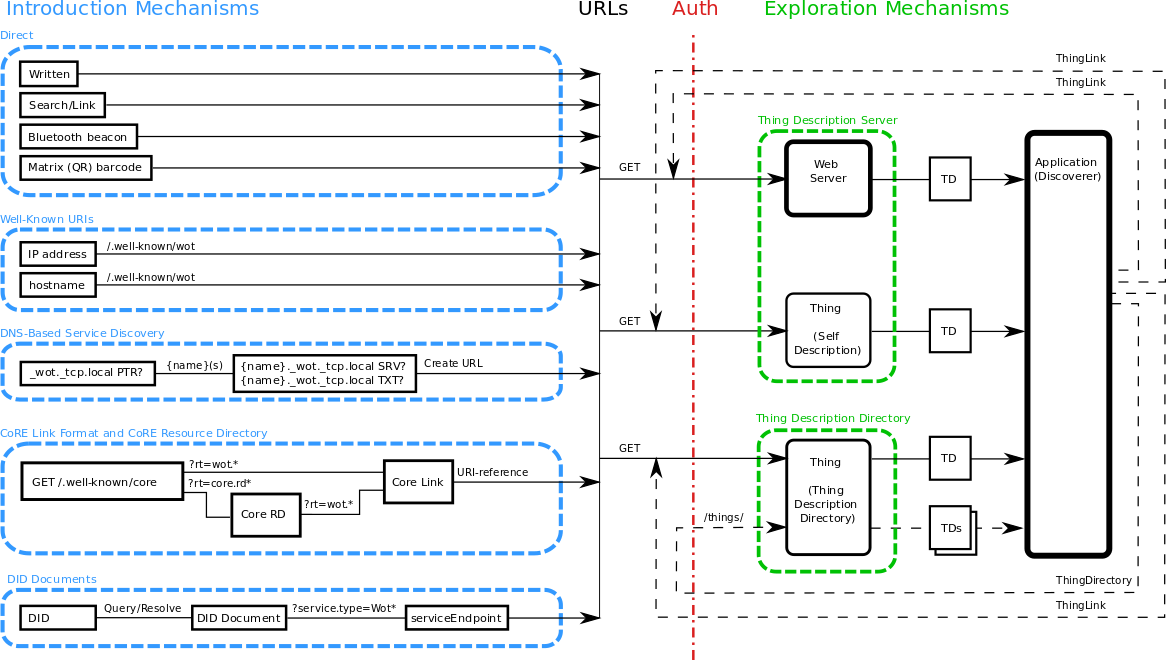
\includegraphics[width=16cm]{discovery-overview.png}
    \caption{Discovery-Architektur}\label{fig:discovery_overview}
\end{figure}

Der \gls{sd} Prozess ist dabei in zwei Phasen unterteilt, die Einführungs- und die Erkundungsphase.
Die Einführungsphase nutzt bestehende Erkundungsmechanismen, um ein oder mehrere \glspl{url} zu erzeugen.
Diese \glspl{url} enthalten selbst keine Metadaten und verweisen auf Erkundungsdienste.
Erst diese Erkundungsdienste stellen dann Metadaten in Form von \gls{td}[s] und \glspl{tdd} bereit.
Dabei gibt es zwei Arten von Erkundungsdiensten:

\begin{itemize}
    \item Ein Dienst, der sich um die Verteilung einer einzelnen \gls{td} kümmert, wie z.\,B.\ ein einfacher Webservice.
    \item Ein Dienst für das Durchsuchen eines \gls{tdd}[s], worin sich mehrere \gls{td}[s] befinden.
\end{itemize}

Der Discovery-Prozess verwendet eine zweistufige Architektur.
Im ersten Schritt generieren die Einführungsmechanismen \glspl{url}, die dann in der Erkundungsphase referenziert und mit Metadaten verknüpft werden.
Die Einführung kann durch jeden Mechanismus durchgeführt werden, der eine \gls{url} liefern kann.
Der Einführungsmechanismus kann dabei auch mehrere \glspl{url} liefern, die in der Erkundungsphase in mehreren \glspl{td} resultiert.
Eine \gls{url}, die von einem Einführungsmechanismus zur Verfügung gestellt wird, zeigt dabei immer auf einen Endpunkt eines Erkundungsmechanismus, der eine \gls{td} liefert.
Dies ist im einfachsten fall eine gewöhnliche Ressource, die von einem Webserver bereitgestellt wird und eine \gls{td} zurückgibt.
Im Sonderfall gibt es noch eine selbst beschreibende \gls{url} für ein \gls{thing}, was seine eigene \gls{td} liefert.

Jeder Client, der eine einzelne \gls{td} mit einer einzelnen \gls{url} abrufen kann, unterstützt \glsxtrshort{wot}-Discovery.
Sie muss dabei aber gewisse Anforderungen erfüllen, wie z.\,B.\ dass mindestens ein Einführungsmechanismus vorhanden sein muss
oder das mehrere Aufrufe desselben Einführungsmechanismus möglich sind.
Diese Anforderungen sorgen dafür, dass genau definiert ist, wie sich die \gls{td} in verschiedenen Szenarien verhalten soll.
Es können verschiedene Einführungsmechanismen verwendet werden, wie z.\,B.\ die direkte Variante über eine \gls{url}, eine Variante mit DNS-basierter Service-Discovery, oder eine Variante mithilfe von \gls{core}.
Das Ergebnis ist aber immer eine \gls{url} eines Erkundungsmechanismus, welcher die Metadaten einer \gls{td} beinhaltet.

Im Erkundungsprozess werden \glspl{td} mithilfe von zwei Mechanismen über einen Server zur Verfügung gestellt.
Jeder Webdienst, der über eine \gls{url} referenziert werden kann und eine \gls{td} zurückliefert, kann als Erkundungsmechanismus verwendet werden und wird als \glsxtrshort{td}-Server bezeichnet.
Ein \glsxtrshort{td}-Server muss dabei nicht zwangsläufig ein \gls{thing} sein, sondern kann auch über ein einfachen Webserver implementiert werden.
\glsxtrshort{td}-Server können auch zur Selbstbeschreibung verwendet werden. Für die Selbstbeschreibung hostet ein \gls{thing} seine eigene \gls{td} und stellt sie zur Verfügung.
Neben \glsxtrshort{td}-Servern gib es noch die bereits erwähnten \glspl{tdd}, worin sich keine oder mehrere \gls{td}[s] befinden und verwaltet werden können.
Für jede \gls{td} enthält das \gls{tdd} zusätzliche Metadaten für Buchführungs- und Suchzwecke.

\subsection{Sicherheit \& Datenschutz}\label{sec:wotsecurityprivacy}

Die Sicherheit eines \glsxtrshort{wot}-Systems kann sich auf die Sicherheit der \gls{td} selbst, oder auf die Sicherheit des \gls{thing}[s] beziehen.
Das \gls{wot} führt keine neuen Sicherheitsmechanismen ein. Es wird lediglich garantiert, dass bestehende Funktionalität und Sicherheit der Systeme beibehalten wird.
Hierbei werden verschiedene Anforderungen gestellt. Bei der Offenlegung einer \gls{td} sollte es z.\,B.\ möglich sein, bewährte Verfahren für die Sicherheit und Integrität anzuwenden.
Eine \gls{td} sollte zudem den tatsächlichen Sicherheitsstatus des von ihr beschriebenen Geräts genau wiedergeben.
Das \gls{wot} kann potenziell auf viele Protokolle angewendet werden. Für die Begrenzung des Umfangs wird sich aber hauptsächlich auf HTTP(S), CoAP(S) und MQTT(S) konzentriert.
Das \gls{wot} stellt zudem ein Framework bereit, welches eine Reihe möglicher Bedrohungen und Sicherheitsziele auflistet, die ein Anwender berücksichtigen sollten.
Des Weiteren werden Sicherheitspraktiken für die Gestaltung einer \gls{td} beschrieben, sowie ein Beispiel für eine sichere Konfiguration vorgeführt.

Mehrere Bedrohungen können die Privatsphäre von \glsxtrshort{wot}-Betreibern beeinträchtigen. Ein Betreiber kann hier z.\,B.\ eine Person sein, die ein Smart-Home besitzt,
oder eine Firma, die mehrere \glsxtrshort{wot}-\glspl{thing} in einer Fabrik betreibt.
Eine \gls{td} kann z.\,B.\ datenschutzrelevante Informationen preisgeben, wie die detaillierte Konfiguration eines einzelnen \gls{thing}[s].
Es können ebenfalls datenschutzrelevante Informationen durch Beobachtung der Kommunikation zwischen einem WoT-Endpunkt (Client, Server oder Gerät) und einer \gls{tdd} ermittelt werden.
Abhängig von der Netzwerktopologie können \glsxtrshort{wot}-Systeme Betreiberdaten zwischen dem \glsxtrshort{wot}-Konsumenten und dem \glsxtrshort{wot}-\gls{thing} über viele Zwischenknoten übertragen werden.
Wenn diese Knoten auf die Betreiberdaten zugreifen oder sie verarbeiten, kann es dazu kommen, dass ungewollt Informationen preisgeben werden.
Zusätzlich zu den oben beschriebenen Maßnahmen ist es wichtig, die Betreiber über die gesammelten Daten zu informieren und ihnen die Möglichkeit zu geben, den Grad dieser Offenlegung zu kontrollieren.

